Bereits im Jahr 1827 war dem schottischen Botaniker Robert Brown aufgefallen, dass Blütenpollen in einem Glas Wasser eigenartige Zickzackbewebungen ausführen. Erst nahezu 100 Jahre später erkannte Albert Einstein, dass die Bewegungen auf fortwährende Stöße der Wassermoleküle zurückzuführen sind. Während Einstein damit ein weiteres Argument für die Existenz von Atomen und Molekülen lieferte, war seine Beobachtung auch eine Evidenz für die molekulare Theorie der Wärme. Die mittlere Geschwindigkeit der Wassermoleküle hängt demnach von der Temperatur des Wassers ab. Erst im Jahre 1926 konnte der französische Physiker Jean-Baptiste Perrin die Brown'sche Molekularbewegung experimentell mit hoher Genauigkeit bestätigen, wofür er auch den Physik-Nobelpreis erhielt.

In Versuch 223 beobachten wir mit einem Mikroskop die Brown'sche Bewegung von in Wasser suspendierten Latexpartikeln. Wir werden die statistische Bewegung untersuchen und anhand der Bahn eines einzelnen Teilchens die Boltzmannkonstante bestimmen.

\subsection{Physikalische Grundlagen}

Als vereinfachtes Modell der Brown'schen Bewegung betrachten wir einen eindimensionalen Random-Walk. Wir stellen uns also ein einzelnes, freies Teilchen vor, welches sich auf einer Linie bewegen kann. Alls $\tau$ Sekunden erfährt das Teilchen einen Stoß, also $n = \frac{t}{\tau}$ Stöße in einer Zeit $t$. Bei jedem Stoß besteht die gleiche Wahrscheinlichkeit $p = \frac{1}{2}$, dass das Teilchen um die Distanz $\delta$ entweder nach links ($-\delta$) oder nach rechts ($+\delta$) verschoben wird. Um nach $n$ Stößen an der Position $m\delta$ zu sein, muss sich das Teilchen somit $\frac{n+m}{2}$-mal nach rechts und $\frac{n-m}{2}$-mal nach links bewegt haben. Um die Position $x = m\delta$ zu erreichen gibt es
\begin{align}
  \binom{n}{\frac{1}{2}(n+m)} = \frac{n!}{\qty(\frac{1}{2}(n+m))!\qty(\frac{1}{2}(n-m))!}
\end{align}
Wege, die das Teilchen gelaufen sein könnte. Die Wahrscheinlichkeit, dass sich das Teilchen nach $n$ Stößen an der Position $x = m\delta$ befindet ist binomialverteilt nach
\begin{align}
  P(m;n) = \binom{n}{\frac{1}{2}(n+m)} p^{\frac{n+m}{2}} (1-p)^{\frac{n-m}{2}}.
\end{align}
Die Wahrscheinlichkeit $p$ für einen Sprung nach links bzw. nach rechts ist für beide Richtungen $p = \frac{1}{2}$. Somit können wir die Wahrscheinlichkeitsfunktion vereinfachen zu
\begin{align}
  P(m;n) = \frac{n!}{\qty(\frac{1}{2}(n+m))!\qty(\frac{1}{2}(n-m))}\qty(\frac{1}{2})^n.
\end{align}

Da das Zeitintervall $\tau$ zwischen den Stößen sehr klein ist, wird $n = \frac{t}{\tau}$ sehr groß. Somit können $n!$ und $m!$ mit der Stirling'schen Formel
\begin{align}
  n! &= (2\pi n)^{\frac{1}{2}} n^n \e{-n}
  \intertext{angenähert und die Wahrscheinlichkeitsfunktion zu}
  P(m;n) &= \sqrt{\frac{2}{\pi n}} \e{-\frac{m^2}{2n}}
\end{align}
umgeformt werden

Wir möchten nun von der diskreten Verteilung der Variablen $m$ und $n$ zu einer kontinuierlichen Verteilung für die leichter messbaren Variablen $x$ und $t$ übergehen. $m$ ist entweder gerade oder ungerade, somit ist $\Delta m = \pm 2$. Betrachtet auf ein Intervall $\qty[x, x + \Delta x]$, kann sich ein Teilchen an $\frac{\Delta x}{\Delta m \delta} = \frac{\Delta x}{2 \delta}$ verschiedenen Positionen befinden. Wir können die Variable $m$ also entsprechend
\begin{align}
  P(m;n)\frac{\Delta x}{2 \delta} = P(x;n) \Delta x
\end{align}
substituieren. Weiter setzen wir $n = \flatfrac{t}{\tau}$, $m = \flatfrac{x}{\delta}$ und führen den Diffusionskoeffizienten 
\begin{align}
  D = \frac{\delta^2}{2\tau}
\end{align}
ein. Damit erhalten wir die Funktion
\begin{align}
  P(x;t)\Delta x = \frac{\Delta x}{\sqrt{4 \pi D t}}\e{-\frac{x^2}{4 D t}}
\end{align}
für die Wahrscheinlichkeit, dass sich ein Teilchen nach der Zeit $t$ im Intervall $\qty[x, x + \Delta x]$ befindet. Setzen wir 
\begin{gather}
  \mu = \expval{x} = \int_{-\infty}^{\infty} x P(x;t) \dd{x} = 0,\\
  \sigma^2 = \expval{x^2} = \int_{-\infty}^{\infty} x^2 P(x;t) \dd{x} = 2Dt,
  \intertext{so lässt sich diese mit einer Gaussverteilung}
  G(x;\mu, \sigma) = \frac{1}{\sqrt{2\pi}\sigma}\e{-\frac{(\mu-x)^2}{2\sigma^2}}
\end{gather}
um $x = 0$ identifizieren. Aus der Definition der Varianz $\sigma$ ergibt sich sogleich die Einstein-Smoluchowski-Gleichung
\begin{align}
  \sqrt{\expval{x^2}} = \sqrt{2Dt}.
\end{align}
Welche besagt, dass der mittlere Abstand eines Teilchens von dessen Ursprungsort mit $\sqrt{t}$ zunimmt.

Diese Gesetzmäßigkeiten lassen sich leicht von der bisherigen eindimensionalen Betrachtung auf höhere Dimensionen erweitern. Es gilt dann für das mittlere Verschiebungsquadrat
\begin{align}
  \expval{r^2} = \expval{x^2} + \expval{y^2}. \label{eq:r_squared}
\end{align}

Durch die Isotropie der Brown'schen Bewegung gilt im zweidimensionalen Fall $\sqrt{\expval{r^2}} = \sqrt{4Dt}$ und im dreidimensionalen Fall $\sqrt{\expval{r^2}} = \sqrt{6Dt}$. Nach Einstein gilt für den zuvor eingeführten Diffusionskoeffizienten
\begin{align}
  D = \frac{kT}{f}.
\end{align}
Dieser gibt die Beweglichkeit eines Teilchens, abhängig von der Boltzmannkonstante $k$, der Temperatur $T$ und dem Reibungskoeffizienten $f$ an. Letzterer lässt sich für kugelförmige Partikel mit dem Radius $a$, suspendiert in einer Flüssigkeit mit Viskosität $\eta$ nach dem Stokes'schen Gesetz
\begin{align}
  f = 6\pi\eta a
\end{align}
berechnen. Es gilt also 
\begin{align}
  D = \frac{kT}{6\pi\eta a}.
\end{align}

Setzen wir dies in die Definition des mittleren Verschiebungsquadrats in zwei Dimensionen ein, so erhalten wir
\begin{gather}
  \expval{r^2} = \frac{4kT}{6\pi\eta a} t
  \intertext{und schließlich}
  k = \frac{6\pi\eta a}{4 T t} \expval{r^2}\label{eq:k_boltz}
\end{gather}
zur experimentellen Bestimmung der Boltzmannkonstante $k$.
\newpage\noindent
\subsection{Versuchsdurchführung}

Wie eingangs bereits erwähnt, betrachten wir in diesem Versuch in
Wasser suspendierten Latexpartikel Mikroskop. Der erste Versuchsteil umfasst die Herstellung der Probe, während es in den nachfolgenden Teilen um die Erfassung der Bewegung, sowie die Eichung der Software geht.

\textbf{Herstellen der Probe suspendierter Latexpartikel.} Bevor wir mit der eigentlichen Messung beginnen können, müssen wir eine Probe auf einem Objektivträger präparieren. Dieser widmen wir uns im ersten Versuchsteil. Hierzu kleben wir ein Stück doppelseitiges Klebeband, aus dessen Mitte wir ein Loch ausgestanzt hatten, auf den Objektivträger. In den ausgestanzten Bereich pipettieren wir ca. $150\si{\micro\liter}$ der Probeflüssigkeit und kleben dann ein weiteres Deckglas darauf, um die Flüssigkeit einzuschließen. Dabei achten wir auf die Vermeidung von Luftblasen in der Flüssigkeit. Wir spannen nun den Objektivträger in das Mikroskop ein. Nach dem Einstellen des Objektivs \textit{100/1.25 oil} verwenden wir den groben und feinen Fokusantrieb des Mikroskops, um die suspendierten Latexpartikel in der Probe zu fokussieren. 

Für alle folgenden Schritte verwenden wir die Funktionen, darunter eine Video- und Bildübertragung, Aufzeichnung und Maßstab-Kalibrierung, der Mikroskopsoftware am PC.

\textbf{Aufnahme einer Bildfolge.} Aus den sichtbaren Partikeln wählen wir einen eher mittig gelegenen aus, um möglichst zu vermeiden, dass dieser während der Messung aus dem Bild wandert. \abbref{fig:bild105} zeigt einen Schnappschuss aus dem Zeitraum der Messung, das beobachtete Partikel ist hier mit einem Kreis markiert. Nun nehmen wir eine Folge von 156 Bildern auf und notieren im Nachhinein noch die Raumtemperatur für die späteren Berechnungen.

\begin{figure}[H]
  \centering
  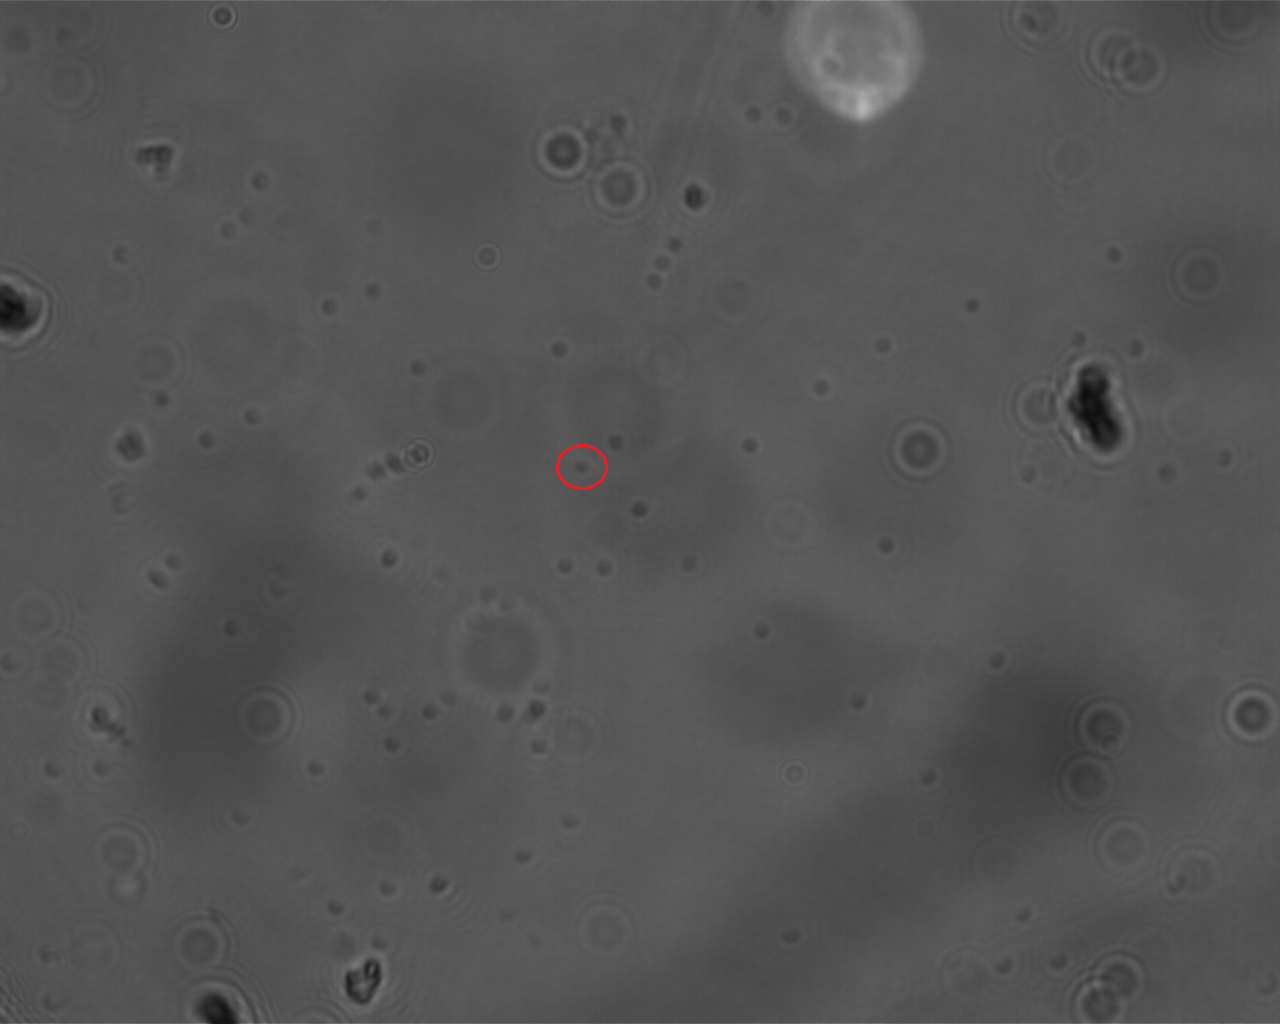
\includegraphics[width=.66\textwidth]{files/Bild105.png}
  \caption{Auszug aus der aufgezeichneten Bildreihe mit dem beobachteten Partikel mittig, rot markiert.}
  \label{fig:bild105}
\end{figure}
\textbf{Eichen des abgebildeten Ausschnitts mit einem Mikrometermaßstab.} Um in der nachfolgenden Auswertung mit den korrekten Längeneinheiten rechnen zu können, nutzen wir einen Mikrometermaßstab, um den Abbildungsmaßstab zu ermitteln. \abbref{fig:calibration} zeigt, wie der Mikrometermaßstab unter dem Mikroskop aussieht. Je zwei Teilstriche auf der Skala sind $10\si{\micro\meter}$ voneinander entfernt. In der Abbildung sind außerdem die beiden Messpunkte zu sehen, welche von der Software zur Berechnung des Abbildungsmaßstabs benutzt wird.

\begin{figure}[H]
  \centering
  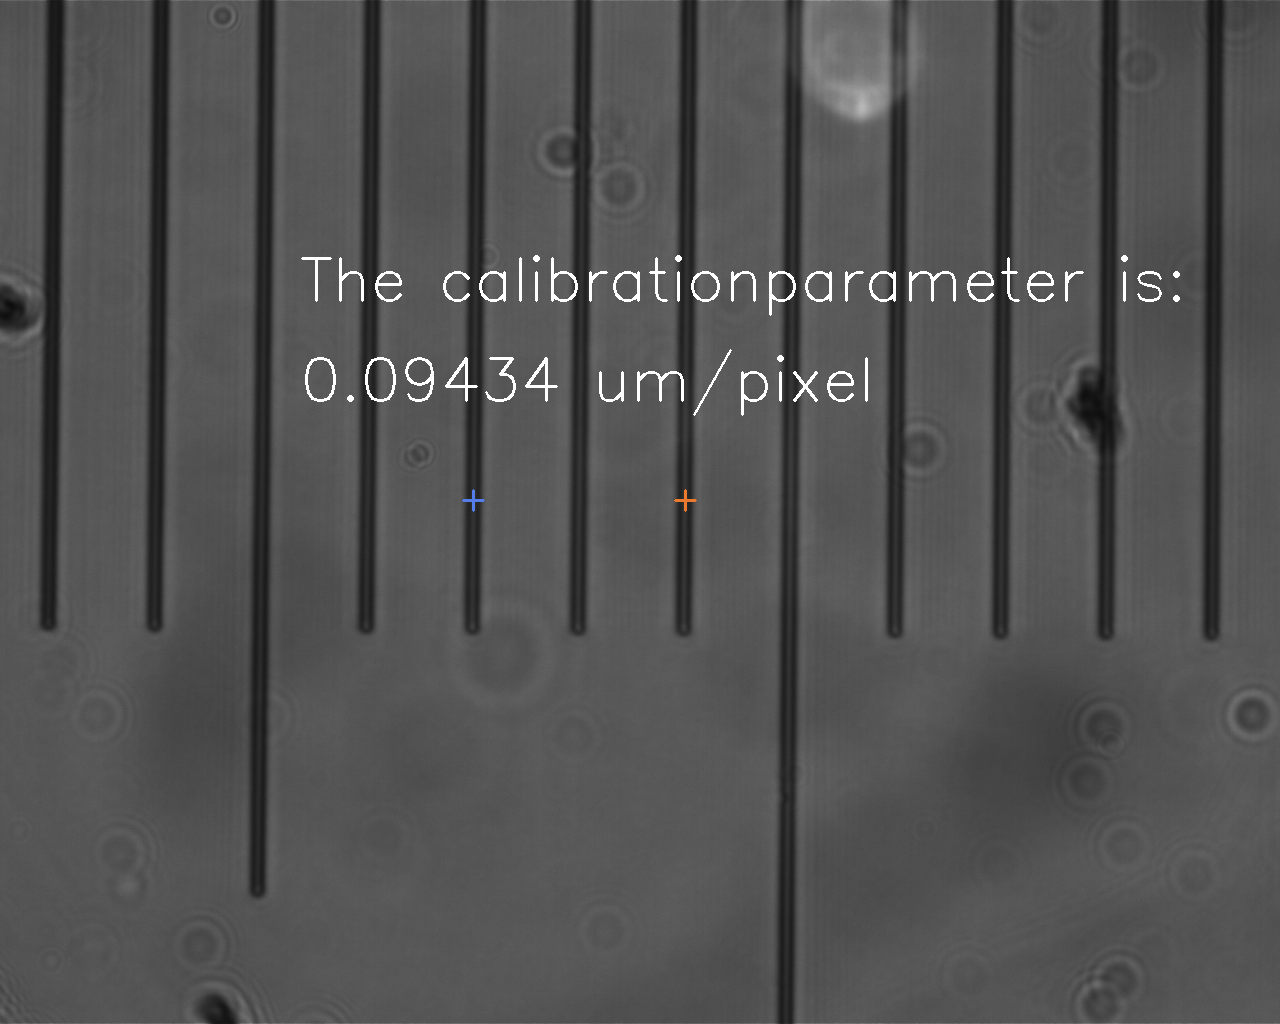
\includegraphics[width=.66\textwidth]{files/Calibration.png}
  \caption{Objektmikrometer unter dem Mikroskop zur Bestimmung des Abbildungsmaßstabs.}
  \label{fig:calibration}
\end{figure}
\textbf{Vermessen der Partikelpositionen für jedes Bild der auf genommenen Folge.} Abschließend müssen wir das von uns zuvor ausgewählte Partikel auf jedem der aufgenommenen Fotos markieren. Hierbei hilft uns zu Teilen wieder die Mikroskopsoftware. Da diese jedoch das ausgewählte Partikel nicht automatisch erkennt, müssen wir diesen für jedes Bild einzeln manuell suchen und auswählen. Die ausgewählten Positionen werden von der Software automatisch in einer Textdatei zur Auswertung gespeichert.